\documentclass[article,twoside]{memoir}
\usepackage{hyperref}
\usepackage{graphicx}
\usepackage[%
    natbib=true,%
    backend=biber,%
    backref=true,%
]{biblatex}

\title{Libertarian Welfare State}
\author{Luis Pedro Coelho}

\addbibresource{references.bib}
\def\thought#1\par{%
    \noindent \emph{#1}\par\bigskip%
}
\let\backnote\footnote
\def\FIXME#1{ FIXME: #1}
\def\epigraph#1{%
\begin{flushright}
\textit{#1}
\end{flushright}%
}

\begin{document}
\maketitle

\begin{quote}
``
There is little reason why the government should not also play some role, or
even take the intiative, in such areas as social insurance and education, or
temporarily subsidize certain experimental developments. Our problem here is
not so much the aims as the methods of government action.''

-- F.A. Hayek
\end{quote}

\chapter{Introduction}

There is a role for the state in guaranteeing everyone a set of basic goods so
that they may fully participate in society as equal citizens. However, the way
in which state institutions go about performing their tasks does not always
respect the recipients of such aid.

Despite all the rhetorical polarization in modern day America, there is big
center on which both the Democrats and Republicans agree. The Democrats are not
socialists (they will not completely nationalize industry) and the Republicans
will not eviscerate the institutions of the welfare state. No matter who wins
the next election, the American government will be about as big as it is now
(at most a few percentage points bigger or smaller).

The question is not whether to have state or not, nor even whether to have a
welfare state or not, but which forms it should take.

There are a few interlocked goals to this book. One is to save the economic
freedom arguments from those who have used them (and often abused them) from
the conservative side.\footnote{For example, conservative activists will often
use the language of property rights to defend zoning laws that keep poor,
dark-skinned, people away from rich people. However, zoning laws are very much
anti-free-market. See
\url{http://www.theatlantic.com/business/archive/2012/03/affordable-housing-and-social-engineering-in-new-jersey/255269/} for a perfect example.} % FIXME: inline the comment

The other is to present free-market solutions to social problems not only as
more efficient than current alternatives (which is often the angle that is
taken), but \emph{as morally superior}. Not morally superior only because they
involve less coercion or better respect property rights (the traditional
libertarian goals), but morally superior because of the way in which recipients
are treated. At the interface of the welfare state and the recipients, there
are no magic ``rights,'' but a real interaction between recipients and
bureacracies. The alternative models I propose here will empower (in the
literal sense of the word, will give power to) the recipients.

A family who approaches a school system with a voucher that gives them choices
is more empowered and will get more respect than a family who, because they
cannot afford a private school, approaches their failing neighborhood school.
In Chapter~\ref{chpt:education}, I will discuss the evidence on school choice
and whether children benefit from switching schools under that system. I think
that there is evidence for a small positive effect, but \emph{even if there was
no effect on grades or other outcomes, school choice would be the more moral
system because it treats recipients with greater respect}. In fact, if the
current system was a voucher system, then I do not think that there would be
very strong arguments against moving to a limited-choice system (currently, in
the US, we can find systems ranging from voucher to assigned school as well as
many systems in between where there is a certain amount of choice, but not
complete choice\footnote{There is always almost complete choice for parents who
can afford it. They can resort to private schools or simply buy a house in
their desired school district. The discussion is only whether that choice
should be extended to not so fortunate parents. We should not lose track of
this simple fact.}).

Too often the focus of welfare discussion is on the demand side, how to pay for
it? This is most evident in health care. Almost all of the discussion on health
care reform in 2008--10 was about how to pay, given a fixed set of resources.
In the health care chapter, we will look at the other side of the ledger, how
to provide services and I will argue that health care costs are so high, at
least in part, due to over-regulation in the provision of services.

The welfare state is a big subject. I will focus on a few subjects: education,
health care, basic income provisions, and the environment. I will discuss how
American institutions currently operate and present alternatives. These will
not be utopian alternatives, but we will see examples from other societies. In
particular, a few societies will keep coming up, the S-countries: Singapore,
Sweden, and Switzerland. Neither is a good model for the US to follow.
Singapore is a dictatorship and, no matter how mild of a dictatorship, its
political system is abhorrent. Still, we can look at some of their economic
policies as examples. Sweden and Switzerland are both democracies, but are
small countries, with a culturally and racially homogeneous population.

It may be the case that a complete rewrite of the system to a Universal Basic
Income as favoured, for example, by \citet{MurrayUBI}, is a much better
alternative. However, my focus here is, to borrow a phrase from the blog
\emph{marginal revolution}, ``small steps to a much better world.''

The free market is a friend, not a foe of the downtrodden.



\chapter{The Curious Asymmetry}

The US government currently consumes about 40\% of total GDP, when you consider
all the levels of government (local, state, and federal).

In international comparisons, too often one sees the US Federal Government
compared with total government spending in other countries. This makes the US
seem like a small-government country. However, in the US Federal system, state
and local governments spend a large chunk of what government
spending.\footnote{It is also noteworthy that many other countries manage their
spending with a federal system or an even more local level, but that is rarely
mentioned in international comparisons.  So, these comparisons really are
apples to oranges.}

If we look just at the economic role of government (which is the focus of this
book), we can place the possible governments from right to left. At one end of
the spectrum, we put the followers of Ayn Rand, exposing anarcho-capitalism. At
the other, we place  full-blown communism with forced labor camps. At the first
end, individuals have all rights and there are no societal rights; at the other
end, individuals have no rights and society owns them as slaves.  Economically
speaking, we are close to the middle of this spectrum.\footnote{On non-economy
dimensions, however, the 20th century has seen a steady walk from the society
to the individual end of the spectrum. I find it the most surprising political
fact of the last 100~years that the anarchists basically won on state
interference on sexuality. The result may not be the sexual utopia that radical
socialists predicted nor the Randian promise of a rational open sexuality (her
own real-life attempts were not as successful as those of the characters in her
novels). However, in policy, we live in anarchy. Despite the
fact that much hurt comes from it and that there is widespread condemnation of
adultery, it is a matter that has become a private and social matter, outside
the boundaries of courts.  This is, however, a topic for another book.} Still,
in polite speech there is too often an idea that we are on the verge of
political anarchy.\FIXME{Get quotes}

Yes, it is true that there are those that accuse Democrats of being Communists
or Nazis. A few signs in Tea Party demonstrations did compare Obama to Hitler.
However, this is not the establishment in the same way that op-eds in the New
York Times or University professors writing widely-read books.

One of the negative side-effects of this discourse is that it allows the
big-government GOP to grab the credit for being small-government, while never
really addressing any of the major interventions that the government has in the
economy. They consistently vote for major farm subsidies, a completely needless
(and costly) intervention in the economy.\footnote{The only element of the farm
bills that consistently gets cut with bipartisan support are the tiny part that
supports school lunches for children. The major cost of the bill comes, of
course, from subsidies to farmers in various guises.}\FIXME{find link to news
items.}


\section{Economic Freedom is Important}

In this book, I ask you to consider economic freedom as an important freedom.
Not all trumping, ``taxation is theft,'' kind of freedom; but something that we
need to respect and be careful when we abridge it. Consider the case of another
basic right, that of free-speech. I could make the following argument:

\begin{quote}
The idea that there is a free-speech right is an illusion. It might make us
feel good, but, upon further examination, we quickly detect the falsehood.
Historically, there has never been completely free speech. We cannot shout
``fire'' in a crowded movie theater and certain forms of obscenity have always
been banned.

Or consider the criminal master-mind who, upon getting arrested, claims that
``yes, he did say that so-and-so should be killed and even offered money for
it,'' but that is purely speech, he did not pull any triggers. Therefore, he
has a First Amendment Right to Free Speech and the charge of conspiracy is a
violation of his rights.

This is absurd. Society has an interest in what people say. Once you accept
this, you see that there is really no difference (except in degree) between
banning libel and banning criticism of elected officials.
\end{quote}

Naturally, we understand that the above argument is bunk. Accepting certain
restrictions to unbridled speech does not mean that there is no right to free
speech. It means that the free speech can only be regulated when equally
important rights are at stake. In institutional terms, this means that free
speech regulation has an extra layer of protection in the form of judicial
supervision that more run-of-the-mill legislation does not.

Valuing free speech does not mean that there are no limits to it, that does
limits cannot change in response to cultural changes (prohibitions on erotic
material are certainly much more relaxed than before), or that there can be
strong and vigorous disagreements on what is and is not an acceptable limit to
free speech (as the Supreme Court ruling in the Citizens United case on
campaign finance made clear, there is not even complete agreement as to what is
speech and what is not).

Yet, in the area of economic rights, too often, it seems that simply pointing
out that there are necessarily limits and have always been limits to economic
rights, means that the concept is meaningless. Instead, I think that we should
interpret the concept of economic rights like we interpret free speech:
violating those rights can be necessary, it can even be a good thing to do (if
it leads to a better society), but there should be a high level of scrutiny
and, unless there are strong arguments for the violation, we should preserve
people's rights.

Therefore, we can talk about economic rights and not necessarily defend Randian
anarcho-capitalism. Similarly, an argument that denies that these arguments are
absolute does not give the state full power to take someone's house and give it
to someone else because that person will pay more taxes.\footnote{In the US,
the government cannot take a single house, but it can take a whole neighborhood
and demolish it to give it to someone who will pay more taxes by declaring the
neighborhood as \emph{blighted}. Thus ruled the Supreme Court in \emph{Kelo vs.
City of New London}.}

\section{The Rabbit Curve}

This is the \emph{Rabbit Curve}:

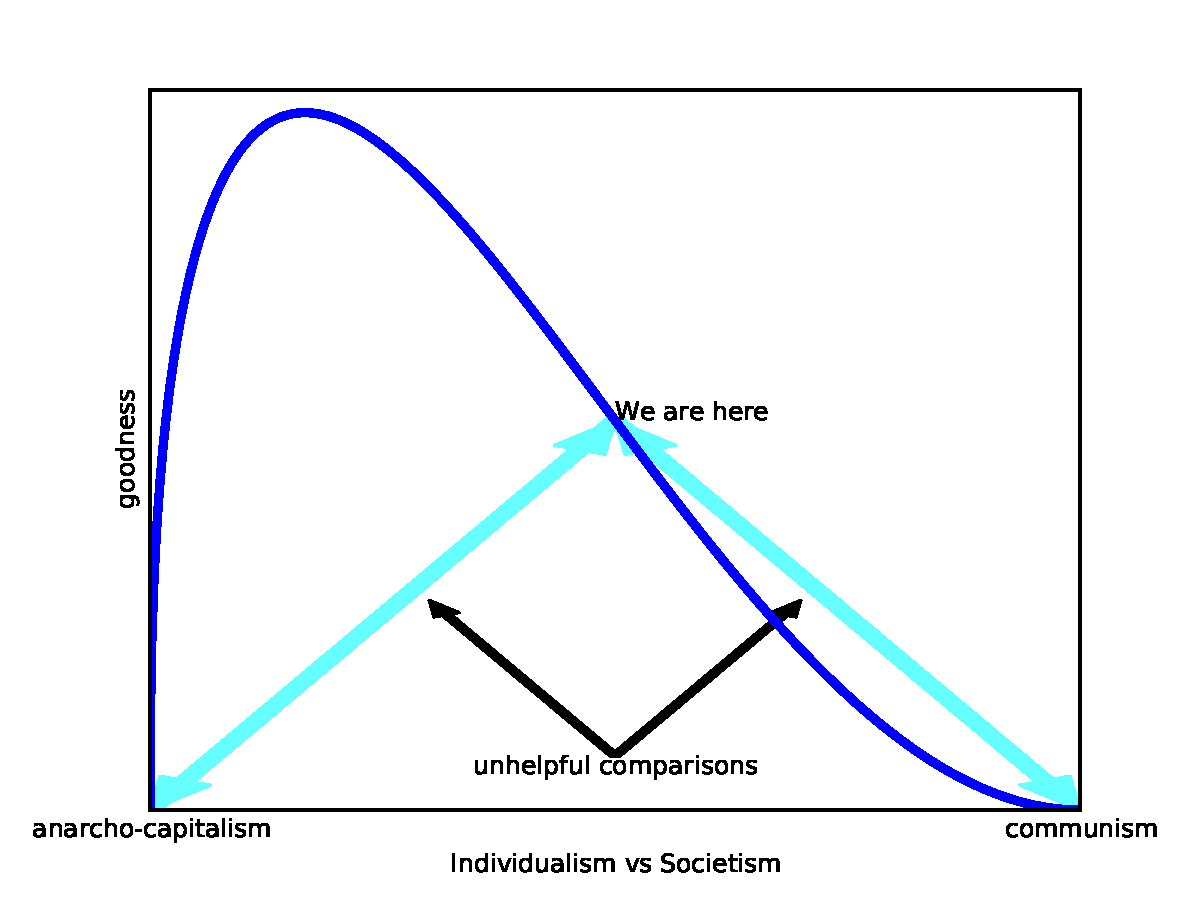
\includegraphics[width=.8\textwidth]{images/rabbit-curve.pdf}

It plots society rights vs.\ ``goodness.'' I could have written
\emph{efficiency} to make it sound more technical.

\subsection{Regulation is Necessary}



\subsection{Curious Asymmetry Thoughts}

\thought Socialism versus anarcho-capitalism is a false dichotomy. Neither is a
choice in front of us right now.

\thought Property rights are not absolute rights, but we still should be
careful not to trampled them for little gain.

\thought We are not on the verge of anarchy.

\thought If X is a problem, we have to address X; not regulate the whole
economy to prevent X from happening.

\thought Regulation vs.\ deregulation is (in the modern political economy)
rarely a useful frame of debate, misregulation is a much more common problem
than either.


\chapter{Education}%
\label{chpt:education}

Universal education is the basis of a fair and decent society (and fairness and
decency are the basis of freedom). Unfortunately, the system has been failing.
At the top of the heap, American education is one of the best in the world; but
its benefits are not spread widely. The education system that an inner city or
poor rural child is forced through is a completely different system from the
one that helps the children of the educated and affluent.

This may sound like bleeding-heart liberalism, which will be followed by a
paean to public schooling. However, public schooling, as it is organized in
most of the United States, does not live up to its ideals. Nor is the
problem simply lack of funding (if it were, it would have been fixed long ago,
as more is spent per pupil now than before).\FIXME{reference for this spending
claim}

Nor is this a diatribe against the public school system as a whole. Most
teachers (but not all) are hard working and many schools are excellent. Most of
the excellent schools, however, are serving the upper-middle class (or the
highly-educated lower earning professionals). And In fact, framing the issue as
public vs.\ private (be it profit or non-profit private) is missing the point.
The point of the critique and the point of the right reforms.

This is about affirming a right to an education and getting there based on what
works and respects the rights of parents and children alike (both of these are
important).

\section{A Right To Education}

In the libertarian literature, there is much discussion of what a right is. In
philosophical terms, much is made of the difference between \emph{positive} and
\emph{negative} rights. Negative rights are those that, simply put, are ensured
if nobody bothers you. You have free speech if you can write whatever you want
without any interference (in the United States, this right is almost
absolute, but not completely). Positive rights are those rights that imply that
other must help you if you need to. A right to education means that someone
must educate you. In practical terms, this normally means that tax dollars are
spent on schools and teachers.

Extreme libertarians deny the second kind of rights, positive rights, as they
deny that you can force anybody else to help you. They may be compelled to help
you out of the kindness of their hearts, there may even be a moral case for it;
however, you may not force them to it (and taxation implies always a threat of
force: if you do not pay your taxes, the court system will eventually tell the
police to take your property away be force). Therefore, conclude some
hard-libertarians, if having a right to something implies that someone else
must be forced to work for you, this so-called right is immoral. If they are
feeling especially dramatic, they may even compare it to slavery.\footnote{Here
is Senator Rand Paul on the right to health-care:

\begin{quote}
With regard to the idea of whether you have a right to healthcare, you have to
realize what that implies. It's not an abstraction. I'm a physician. That means
you have a right to come to my house and conscript me.

It means you believe in slavery. It means that you're going to enslave not only
me, but the janitor at my hospital, the person who cleans my office, the
assistants who work in my office, the nurses," Paul said, adding that there is
"an implied use of force.
\end{quote}

This was cited (very critically) by Matt Welch in
\href{Reason}{http://reason.com/blog/2011/05/13/rand-pauls-slavery}, an
assumedly libertarian magazine.}

As usual, I can intelectually understand the position of the hard libertarian
and even see some cautionary value in it. We have to be careful not to assign
too many positive rights lest we sacrifice too much liberty. However, a
cautionary tale tells us to be careful when we go out in the evening. It does
not tell us never to go out.

Schooling is one of those positive rights that I accept wholeheartedly as the
beneficiaries are children.\footnote{Their parents benefit too, of course, but
they are not the main beneficiaries. In fact, we should be wary of catering too
much to the parents who just want a babysitter.} Children have a right to
education and it should be provided with taxpayer resources.

However, I do not think that this implies a need for the public school system
as it is currently organized in most of the United States.

\section{School Choice}

The most obvious alternative to the current system is a voucher-based
mechanism. In this system, parents can choose which school to send their kids
to and the schools receive funding proportional to the number of students they
attract. At the opposite end, we have the assigned-school system where children
attend a school that is assigned to them by the state. This assignment is
normally based on their home address, but sometimes other factors too.

We must realize that currently in the United States, because schooling is a
local rather than a federal issue, there is no single school system and there
are almost pure voucher systems and almost pure assigned-school systems, but
most places are somewhere in between. Within the public school system, parents
often have some choices, but not too many. It would actually be possible to
have complete school choice with only public schools.

Better off parents always have choices.\footnote{Milton Friedman wrote that
``[o]ur views in these respects are, I believe, still dominated by the small
town that had but one school for the poor and rich residents alike. Under such
circumstances, public schools may well have equalized
opportunities.''\backnote{The Role of Government in Education from
\emph{Capitalism and Freedom}, Milton Friedman, 1962.}} They choose in many
ways. Firstly, they live in neighborhoods served by good public schools. These
are, generally, the more expensive neighborhoods in a city (they are often even
outside the main city area, in the poshier suburbs). Alternatively, they can
opt out of the public system completely and send their children to a private
school, including one that caters to their educational biases and
preferences (be it religiously inspired schooling, musically-oriented, or
free-range Montessori). Some even opt out of traditional schooling completely
and home-school their kids. Home schooling used to be an enclave of the
religious fanatics who objected to the study of evolution or sexual education,
but has recently become a viable option in some places such as New York City
whose public schools are notoriously bad.\backnote{\emph{The Homeschool
Diaries} by Paul Elie, The Atlantic, October 2012,
\url{http://www.theatlantic.com/magazine/archive/2012/10/the-homeschool-diaries/309089/}.
Also, \emph{Homeschooling, City-Style} by Lisa Miller in New York, October
2012,
\url{http://nymag.com/guides/everything/urban-homeschooling-2012-10/}.}\footnote{Estimates
say that there are about the same number of children being home-schooled as
attending charter schools in the US.\backnote{\emph{Keep it in the family}, The
Economist, Dec 22 2012.\href{available
online}{http://www.economist.com/news/united-states/21568763-home-schooling-growing-ever-faster-keep-it-family}.}}
The better off parents have choices. The question is only whether we should
extend these possibilities to those parents whose incomes are not as high.

I agree with critics that say that ``school choice is not a panacea.'' But, who
ever said it was, or that it had to solve all problems to be a good idea? It
just has to be better than the alternatives. I could just as easily argue that
``assigned-schooling has not solved all problems,'' because it has not.

\subsection{What Are Vouchers?}

My father-in-law once got into an argument with a ticket inspector on a
Portuguese train. Like is the case in the US, passenger trains in Portugal are
run by the state (they are better than Amtrak; admittedly, a low bar). Finally,
my father-in-law asked: ``is this how you treat your customers?'' The reply
came quickly ``you are not a customer, you are a user of the service.'' My
father-in-law said he then understood there was no hope of getting better
service.

When you approach a large institution as a customer, you do not always get a
good deal. But, at the very least, you can always leave. When you approach them
as a ``user,'' you have no leverage.

You may think that this is very different from the way you are treated in your
dealings with the public school system. But, then again, you are probably at a
school you chose (through buying in the right neighborhood). Because if they
treated you wrongly, you'd leave.

\subsection{School Choice and Public Schools}

Here is a reader's comment on a recent edition of The Atlantic\footnote{The
comment is available at
\url{http://www.theatlantic.com/magazine/archive/2012/12/the-conversation/309177/}.
The original article is at
\url{http://www.theatlantic.com/magazine/archive/2012/10/a-national-report-card/309087/}.}.
Nicole Allan, the original author had argued that the improved schools in New
Orleans were due to the hits against the teachers' union and reform. J. David
Young, the reader replies:

\begin{quote}
    [T]he colorful bar graph does not provide a comparison between the public
    schools and the charter schools today, but only a comparison of the schools
    then and now. The public schools may in fact be better than the charters.
\end{quote}

This is missing the point of choice and vouchers!

In fact, many supporters of choice make the same mistake. The point is not that
voucher schools are better than public schools, or that privately run schools
are better than public schools in general. The point is that, \emph{with
choice, every school is better}. If the reader is correct and the public
schools in New Orleans are now better than the charter schools and much better
than they were before reform, then this is \textbf{an even stronger} argument
for reform.

Most of the school choice studies make this exact mistake: they compare the
kids who attend charter schools with the kids left behind at public schools.
However, the public schools are not a good control group. They are competing to
be better in a way that they would not if the charter schools did not exist.

Or consider the following comment,taken from a long article on the public
school system in Finnland\backnote{``15 Reasons Reformers Are Looking to
Finland'',
\url{http://www.onlineuniversities.com/blog/2012/08/15-reasons-reformers-are-looking-finland/}},
a system which, by some measures, is the best in world: ``Finland offers school
choice, too; the only difference is that all the choices are the same''
This is still missing the point, \emph{because you have choice}, these schools
are not the same as the schools you'd have if there was no choice!


\subsection{More Flexible Schools}

The public sector is over-regulated in the United States\backnote{Robin Hanson
in \emph{Overcoming Bias} at
\url{http://www.overcomingbias.com/2013/06/is-govt-over-regulated.html} who
notes that ``this view suggests that being pro- or anti-regulation isn’t the
same as being pro- or anti-government.'' The context are public schools in
Finnland which combine flexibility and choice.}

\section{Testing}

% FIXME Consider removing this section of turning it into a single paragraph

One issue that shows up with school choice is testing. Logically, they are
completely separate issues. You can have intense testing in a purely assigned
school system and no testing in a school choice system. In fact, with choice
you will need less testing as we expect that parents will know whether the
school is doing a good job and at least some of them will use their increased
power to steer the school.

However, it is certainly the case that testing does show up sometimes in
connection with choice. For example, the Bill and Melinda Gates Foundation is a
proponent of both choice and measurement.\footnote{Tellingly, they are
proposing a very different sort of measurement and testing than what is
typically done: they are proposing, for example, that teacher effectiveness be
evaluated by other teachers who then coach and mentor struggling ones. Another
of their favorite ideas is that students grade their teachers. This is very
different from having students sit through hours of of multiple choice
questions.\FIXME{ find Atlantic links \& original research.}}

I think that testing has become \emph{too much of a good thing}. Some testing
does allow everybody to have an approximate idea of how well the students are
doing and I find the \emph{zero testing} radicals a bit too extreme. Testing
helps the students understand what is important and what is not and it even
helps them learn. \FIXME{find links to research on this.} However, in many
American schools, testing has gotten out of hand and wastes too much of
the student's time on testing.

I do not find the problem of \emph{teaching to the test} to be a very large
problem \emph{per se}. If you have thought a class, especially to
high-schoolers, you probably have had the dispiriting experience of finishing
an inspired explanation, asking for questions and getting a single one: ``will
this be on the test?'' If you want to teach something, you should test for it.
I also think that it is possible to test for much more than typical tests do.
Unfortunately, the testing format does encourage dumbing down the curriculum to
make it easier to test: it is easier to test a series of multiple-choice
questions rather than a long-form essay.

\subsection{School Choice Thoughts}

\thought It's not about private vs.\ public. It's about choice and competition.

\thought The biggest effect of school choice is that it improves public schools.

\thought If charter schools are not that much better in terms of test scores
(perhaps even showing no effects), but parents and students overwhelmingly
prefer them; we should allow them.

\thought Better off parents already have complete choice (through choice of
neighborhood or opting for non-public schooling), the question is whether to
extend this to all parents.

\thought School choice advocates were wrong to get mixed up in the testing
imbroglio. Choice actually weakens the case for testing.


\chapter{Health Care}
\label{chpt:health}

Healthcare is perhaps the major topic that comes up with respect to the welfare
state. Perhaps because it is one that affects us all. Even if we are not sick
now, it is a certainty that we (or a loved one) will be at some point in our
lives. It also seems to strike independently of our actions. We do have some
control over the probabilities: a proper diet, avoiding sedentarism and
smoking. However, our control is only over the probabilities, the dice can
always come against us or anybody.

Much has been written about healthcare in the United States, especially over
the last few years with the passage of the Affordable Care Act (aka Obamacare)
and its step-by-step implementation. Each little step is scrutinized, with
minor changes being trumpeted as heralding a whole new world and every misstep
proving that the whole project is a failure. The only thing that is clear is
that the topic will continue to be active ovver a long time.

However, strangely, there has been little thought given to how to expand the
amount of health care provided. It is all about shuffling resources around, not
about creating more health care.

As the wonks say, the discussion has all been \emph{demand side} (who should
pay? how? when?) and not \emph{supply side} (who should provide services? how?
how to get more services provided?). This chapter will discuss how removing
obstacles to the provision of health care can result in cheaper healthcare, by
sacrificing the frills and using technology so that medical quality can be
maintained.

\section{Why is health care so expensive in the United States?}

Health care is expensive in the United States and it is not clear that
Americans are getting their money's worth. It is not clear that they are not,
either. It is very hard to compare health care results. We can compare health
outcomes, but most health outcomes depend most strongly on lifestyle choices.
Americans do not, on average, make the healthiest choices while eating, and
tend to live overly sedentary lives; until recently, they would smoke more than
almost everybody else too.\footnote{Even as I'm writing this, in 2013, the
levels of smoking in the United States are still at \FIXME.} They also drive
more, especially as teenagers, which shows up in the mortality statistics.
While the effects of widespread availability of guns on crime-related deaths
may be debatable, its effect on suicides is not. None of these factors are
related to health care.

Most other industries are dominated by \emph{almost as good and so much
cheaper} competition. Health care is dominated by \emph{just slightly better
and so much more expensive} competition. We need to focus on the first kind of
competition. To the extent that the extra benefits are not medical, but rather
luxury (plus waiting rooms) or feel-good (over educated doctors taking care of
routine issues), we should be happy to see them go and be replaced by cheaper
medical services.

There are two types of consumers of healthcare: the healthy and the sick. By
healthy I mean both people who are just looking for wellness services or
screening as well as people who are momentarily sick, but will soon be cured.
Of course, we may move from one group to the other (unfortunately, it is easier
to move from healthy to sick, but the reverse also happens). The needs of
these two groups are very different and we have to be careful not to sacrifice
one to the second.

Low deductibles certainly benefit the healthy, but the value of the deductible
is not a big consideration for a chronically sick individual; while the overall
cost is (and high deductibles can arguably lower the overall cost).

\section{Is the US healthcare system ``free market''?}

No, and the idea that it is is one of the most unhelpful ideas in the whole
debate. When I say that the system is not free market, I do not mean that the
system is not a perfect free, idealized free market. I mean that the healthcare
sector is one of the most heavily regulated, subsidized, and heavy-handed
managed in the United States. Therefore, to argue that its many failings (and
there are many failings, for sure) somehow show that the free market cannot
provide good healthcare is borderline ridiculous.

In fact, the US government \textbf{spends more on healthcare than other
\emph{so called socialist}\footnote{As I argue throughout the book, but
particular in Chapter~\ref{chpt:international}, many countries in Northern
Europe are not socialistic, but at least as free-market as the United States.}
healthcare systems}. This is without even counting the largest component of
government spending on healthcare: the tax deduction
on employer provided healthcare. If you add this component, then \emph{the US
government spends more on healthcare than any other developed country}. This is
not the hallmark of a free market. % FIXME Add numbers. Tables

The problem is not that the government is not involved in health care, the
problem is that it is involved in number of very negative ways (certainly also
in positive ways, but rarely is it uninvolved).

In fact, I think that there should be more pressure on free market economists
to explain why the US healthcare system actually works pretty well given this
deep involvement of the state.\footnote{This is partially tongue-in-cheek, but
I think this way to pose the problem has a lot of truth in it. My answer is
that health care is a highly desirable good. Therefore, people are willing to
pay the higher costs for all the extra layers and all the inefficiencies. The
cost of the state involvement does not appear in worse outcomes for most
people, but in higher costs for everyone and reduced access for a minority.}

The major feature of the American health insurance system, namely its linking
of coverage to employment is a result of government intervention. This is
one of those cases where there is wide agreement between left-wing and
right-wing researchers that this should be changed, and there is wide agreement
between left-wing and right-wing politicians that this should not be touched
(and it shows how much of the bitter opposition of Democrats and Republicans is
staged). Obama repeatedly stressed that the health care reform he supported
would not impact anyone who already had health insurance.\footnote{As many
politician promises, this one contained enough truthiness to not be an outright
lie, but it was not really kept. According to the law, your company was allowed
to keep offering you the same health insurance as before, you would be
grandfathered in and would not be affected by any of the new regulations. Most
companies, however, decided that it was not worth the hassle of keeping two
sets of plans, one for the grandfathered clients, pre-Obamacare; another one,
which was Obamacare-compliant (in fairness, it was not very clear in exactly
what conditions they were allowed to do that, as they would then not be able to
make any changes in the plan). So, in fact, almost nobody will be able to keep
their health insurance as it was.}

In many markets in the US, to open a new hospital, you need the permission of
the existing hospitals.\FIXME{Cite something here} This is as far from a free
market as you can possibly get: it is using the government to impede
competition, to build a cartel. It is no surprise that new hospitals will not
get approved very often and that there is little competition for low prices.

Naturally, the entry into the medical profession is also regulated by the
government. In fact, Congress more or less decides how many doctors to train
each year. Which is to say, how many doctors will enter the profession that
year. They do this as they decide how many residency slots will be sponsored by
Medicare. As the residency experience is required for the practice of medicine,
this decides how many doctors will enter the profession. Although the
bottleneck is at this level, if it were larger, we would expect that medical
schools would soon start to train more doctors as well.

As usual, I am not arguing for a complete deregulation of the doctors,. It is
probably a good idea that there be certain checks on who can call themselves an
MD and practice medicine.\footnote{Although it is a good example of status quo
bias how we, at the same time, find it normal that quacks of all kinds be
allowed to perform sort-of-medicine as long as they do not call it medicine. A
homeopath can claim to heal any disease with his magic water, often making a
living off exploiting the sick, and we find it completely normal.} However,
there can be too much of a good thing. The smart premed who just misses his
entry into med school would probably become a fine doctor if we gave him a
chance.

The often cited fee-for-service model is also a consequence of how the
government reimburses Medicare and Medicaid providers.

\subsection{But it is the most free market system, right?}

You might be thinking that ``even if the US is not so free-market, it is more
free-market than other countries.'' No, not really. Many other developed
countries have systems which are arguably more free-market than the US.

Again, other countries have less government spending on healthcare, they will
have fewer impediments to doctors practicing.

It is true that the system is often potraied as free-market by both its
defenders and its detractors. During the debates on health care reform, one of
the oft quoted lines from some of the more ignorant opposers was \emph{Keep
your government hands off my Medicare}. This is absurd: Medicare is a
government run program\footnote{And, no, I do not believe that the protestors
were arguing for a libertarian welfare solution of deregulating Medicare. Not
even in an unconscious way.}. This just another example of how free-market
rethoric is coopted and used to mean and advocate for decidely non-free-market
things. It actually points to the fact that healthcare in the US is already
mostly government run.

\section{Can the government buy healthcare?}

A common argument for heavy government intervention into the healthcare market
is that a market in healthcare is impossible for behavioral reasons: people do
not behave according to rational self-interest when it comes to health and this
makes the resulting market be skewed.\footnote{This argument has a strong
pedigree, it goes back to an article from Nobel laureate Kenneth Arrow,
published in 1963. In a restyled form, it is now very common in the mainstream
press.}

The reason is that health care is different from other markets. Anyone
can easily compare the price of apples or gas and it is something that we buy
on a regular basis and therefore can respond to bad service productively: this
means purchasing more from the good providers, which will grow while the bad
providers will need to change their behaviour or lose market share. However,
major health purchases are made in a situation of distress.  If they are made
for family members, then it is morally difficult for a family member to perform
a cost-benefit analysis. Therefore, as individuals we choose badly when it
comes to health care.

However, it does not immediately follow that the government can do a better
job. We can ask the same question about government deciders: can they make
rational decisions in the context of healthcare? After all, government decisors
are people too and their motivations are not rational self-disinterest. The
political/bureaucratic process has its own behavioral blind-spots. They
naturally differ from the blind spots of the individual, but are they any less
harmful?

For example, in 2008, the FDA conditionally approved Avastin for use in breast
cancer. What this means is that it was still experimental, but there was enough
hope that it would have a positive effect in patient's outcomes that it was OK
to let the general patient population have access to the medication while more
studies were being conducted to confirm. Unfortunately, it turned out that
\emph{Avastin is actively harmful for breast cancer
patients}~\cite{avastin-harfmul}\footnote{See this note in Science magazine:
\url{http://news.sciencemag.org/scienceinsider/2011/06/breast-cancer-drug-gets-a-unanimous.html}}.
The problem is that it seems that Avastin has no effects on the cancer, but it
has strong negative side-effects.

This led to a strong outcry. Those outcrying were wrong, of course, but this
fact did nothing to diminish their emotional appeal. Cancer survivors who had
taken Avastin appeared at televised hearings in tears (of course, thanks to
\textbf{other} drugs, many women now, thankfully, survive breast cancer; but
this is unrelated to Avastin).\footnote{See this note in the HufftingtonPost:
`` 'It's saved my life,' said a tearful Sue Boyce, 54, of Chicago.''\backnote{
\url{http://www.huffingtonpost.com/2011/11/18/avastin-breast-cancer-fda-approval-revoked_n_1101468.html}.}}
Families of current patients and the patients themselves spoke about being
scared this drug will be taken away. The political system quickly responded and
provided guarantees that Medicare would continue to cover (pay for) Avastin.
Avastin costs 100,000 dollars a treatment and it hurts patients, but Medicare
rushed in to provide it at taxpayer expense.

This is not just one isolated incident. As we discuss in more detail below, the
problem is more profound: every time a government regulator stops a good
solution, the victims are invisible or seem unconnected to the regulation; so
there is little penalty in making this sort of mistake. On the other hand, if
it ever allows anything that is later revealed to have been a mistake or even
possibly a mistake, then there is an outcry. Therefore, \emph{government
regulators should be expected to be very risk adverse}.

A separate issue with government regulation (particularly in the American
political system), is that it responds strongly to well-organized pressure.
This leads it to cave to interest groups that manage to garner both money and
sympathy. This is particularly true if it is regulating what others must spend.
Here are a few other completely unscientific treatments that the political
system has required be covered by private health insurance:

\begin{itemize}
\item dolphin treatment
\item acupuncture\backnote{\emph{Acupuncture as ‘essential’ health care?
California weighs the question} by Sarah Kliff, Washington Post Wonkbook blog,
September 1, 2012.
\href{link}{http://www.washingtonpost.com/blogs/wonkblog/wp/2012/09/01/acupuncture-as-essential-health-care-california-weighs-the-question/}.}
\item homeopathy?
\end{itemize}

Tyler Cowen likes to point out that ``mandates don't stay
modest.''\footnote{This implies an argument for public provision which I find
rather strong: the government as a provider has a stronger interest not to
provide overly expensive treatments; while as a regulator, it can mandate them
as the political/media system suffers from a blind-spot in this area as it
fails to immediately point out that the cost will come out of rising premia.}
Furthermore, as David Goldhill remarks, \emph{health insurance companies
benefit from mandates}. While they may wish to keep their current payments low
(and thus fight having to cover a specific treatment), over the long term, the
more coverage they are forced to provide the better for them as this will be
passed on as premia (because all insurance companies are bound by these
mandates, competition will not keep prices low).

This just shows how the typical narrative of a courageous legislature imposing
a mandate on an unwilling insurance industry has it backwards. To misquote a
diplomat, lobbying is the art of having the legislation you want imposed on
you.\footnote{The original quote reads ``diplomacy is the art of letting
someone have your way'' and is attributed to Daniele Vare, an Italian diplomat
and novelist.}

The reverse is true for individual incentives. We all want to get the most of
the insurance we already paid for. We want to argue and fight for that little
extra benefit. Note how even the language tricks us: everything that an
insurance pays for is called a \emph{benefit}, even if it does very little for
our health. Over the long-term, though, whatever is spent, even if of dubious
medical value or sold at inflated prices, will come out of our pockets.

Can the political system sustain a system of long-term innovation or will it
fall into the temptation of killing the goose that lays the golden eggs? The
FDA already errs on the side of too much caution and not enough innovation.

As with many other governemnt provided services, the government bureacracies
will tend to treat certain kinds of beneficiaries better than others.
Recently, the first Obamacare forms appeared. They are 21~pages and resemble a
tax form. As Megan McArdle pointed out, ``since the whole point is to award
subsidies on the basis of your income, that's not exactly
surprising.''\backnote{\emph{Applying for Obamacare Subsidies Will Be as
Complicated as Doing Your Taxes} by Megan McArdle in The Daily Beast
\url{http://www.thedailybeast.com/articles/2013/03/14/applying-for-obamacare-subsidies-will-be-as-complicated-as-doing-your-taxes.html}.}
While some of the complexity may be inherent to the system, it does itself form
a sort of filter. It privileges those who are better able to deal with complex
forms.\footnote{Non-money elites (journalists, academics, or any other
high-status, low-pay professionals) are often suspect when they promote more
government involvement. They are the ones who will most able to capture the
bulk of government benefits. They will be able to get information on which
benefits are worth it, and apply correctly. They will also be better treated by
public workers than other beneficiaries.\FIXME{Look up study that upper
middle-class gets better drugs from doctors in British NHS.}}

To summarize:
\begin{itemize}
\item The government is too responsive to emotional appeals by well-organized
groups of patients, independently of whether science is on their side.
\item The government takes into account the interests of existing suppliers.
\item Government services often exhibit an inequality of access that is
non-monetary, but no less real and damaging.
\end{itemize}

Maybe individuals are not the best customers of health care, or of anything for
that matter. They may still be the best we've got. Remember the DC dictum:
\emph{those who do not sit at the table, find themselves on the menu}. And
individuals rarely get to sit at the table.

\subsection{Should it be easier to practice medicine?}

This is one of those issues that instinctively leads to false dichotomies. I am
not proposing that anyone should be allowed to perform open heart surgery
without any control or that we should have no barriers to the provision of
medical services. However, we can have too much of a good thing. Think,
however, of the premed students who almost made it to medical school, but not
quite. They were surely ``doctor material.''

One of the interesting (if that is the right word) aspects of current
regulation is that it is perfectly legal to sell fake cures. Many quacks
legally get rich offering fake cures. They call themselves ``homeopaths'' or
``naturopaths'' and happily take the money of sick people while steering them
away from the medical services that could help them.\footnote{Many, even most,
homeopaths know the limits of placebo and will steer their patients to medical
care in the case of serious disease, but it is still legal to claim that some
fruit juice cures cancer of HIV.\FIXME{Quote. Mention Steve Jobs?}}

\subsection{Does the FDA save or lose lives?}

Obviously, it does both. We want to make it do more of the saving and less of
the losing, however.

% Tiago Queiroz points out that a lot of innovation follows another pattern:
% initially very expensive, then costs come down
A lot of innovation follows a familiar pattern, the first versions of anything
do not work very well, but are much cheaper. It's \emph{90\% of the effect and
10\% the cost}. Then, as the technology improves, the quality of the new
techniques will often not only match, but overcome what was possible with the
older technology. In medicine, most innovation, however, is \emph{10\% better
at 10 times the cost}. These are not just the musings of extreme
anarcho-capitalists. Michael Mandel at the Progressive Policy Institute has
made exactly these points in a brief on healthcare
(\url{http://autismcrisis.blogspot.pt/2007/08/autism-and-aba-in-uk-controlled-trial.html}).

Still today, Vioxx is often brought up as a scandal and a failure of
regulation. However, Vioxx was not that awful: all pain drugs have terrible
side-effects, Vioxx was oversold as not having any, which was not true, but it
is no worse than any of the alternatives.\footnote{Still today, there are
arguments that \emph{Vioxx should be put back on the market} as some patients
might be better off managing the risks associated with it rather than go
without it. This is tangencial to my point, but I want to point out that the
idea can be defended.} Furthermore, even if we accept that Vioxx should not
have been sold, we need to be careful not to over-react to any mistake that is
only found a posteriori.

\section{Importing Healthcare}

One way in which the United States could lower its health care costs is by
importing more of it. There are several ways in which healthcare can be
imported: below we discuss the idea of bringing more foreign-educated doctors
into the United States, but it can also be made by having American patients
travel to cheaper destinations for care.

While in the past, this may have triggered images of insalubrious surgery in a
third-world country, many hospitals in the rich countries of Asia or Europe can
provide quality service at a fraction of the cost.

Recently, a robot-doctor gained approval in the United States. This is still
being touted as being centered on remote presence, which is a great way to get
doctors to hard-to-access regions.

% http://www.businesswire.com/news/home/20130124005134/en/FDA-Clears-Autonomous-Telemedicine-Robot-Hospitals

\subsection{Importing Healthcare Workers}

A study from the University of Virginia estimated that ``several US states
could solve physician shortages entirely by eliminating the additional
licensing requirements imposed on foreign educated
physicians.''\footnote{``Doctors With Borders: Occupational Licensing as an
Implicit Barrier to High Skill Migration'' by Brenton Peterson, Sonal S.
Pandyam, and David Leblang.}

Note that this would also open an avenue for Americans who could study abroad
for medical school. Already some do, but if it was easier to do so and return
home to practice, many more would perform this end-run around the high cost of
an American medical school.

\subsection{Consulate Care}

I end this discussion on \emph{importing healthcare} with a semi-whimsical
suggestion by George Mason polymath Robin Hanson: consulate care. To quote from
his blog \emph{Overcoming Bias}:

\begin{quote}
Let countries like Sweden, France, etc. with approved national health care
systems have bigger consulates, and open them up to paying customers for
medical services. For example, you could sign up for Swedish Care, and when
needed you’d go to their consulate to get medical care as if you were living in
Sweden.
\end{quote}

Although probably not something feasible (on both political and practical
grounds), this is an interesting thought experiment.

\subsection{Going Abroad for Healthcare}

A simple solution for the issue that health care is cheaper outside the US than
in the US is for Americans go go abroad for it.

\section{Automating Healthcare}

We have discussed how certain tasks could be performed by someone with less
than a medical degree and how this process is already going on the in US with
nurse-practicioners. The ultimate form of down-crenditialing is automation.

When we replace an interaction with an expensive professional with an
interaction with a computer system, the costs for the user can be much lower.
Again, this has already taken place to some extent as websites such as WebMD or
Medline Plus from the National Institutes of Health have provided educated
persons with the possibility to check many of their symptoms and sometimes
replace a call or a doctor's visit.

In a recent edition of The Atlantic, Jonathan Cohn claims that ``nobody expects
American patients accustomed to treatment from live human beings to tolerate
such a sudden shift for much of their care.''\backnote{\emph{The Robot Will See
You Now} by Jonathan Cohn in The Atlantic, March 2013.} Of course not. Unless,
of course, you give them the choice and expose them to the costs thereof. The
robot being much cheaper, the cost for the patient will be much cheaper. In
fact, as long as patients are insulated from spending choices, we will expect
that they will not tolerate anything but what they perceive to be the best.

An auxiliary argument is that doctors play a role that is not just
physiological, but psychological. They do not only diagnose, ask for tests, and
prescribe remedies (pharmaceutical or otherwise); but they also play a human
role: they comfort and reassure.\footnote{Often, this is tied to a notion that
such comfort is also a form of healing, through the placebo effect. While the
placebo effect is, in fact, real, its effects are often exagerated as well. It
is often confused with the no-treatment effect: that is, for all but very
serious conditions, people tend to recover on their own. A second effect is
that the placebo effect is measurably greater for self-reported measures of
feeling than for physiologically measurable variables.} All of this is
undoubtedly true, but then the question is whether you really need someone with
over ten years of training, and in short demand, to serve that role. As it
stands, many people are already choosing to have some interactions with less
well-trained practicioners who we can afford to pay for longer session. For
example, the resource to midwives or doulas by pregnant women is very often
motivated by the fact that it would be very expensive for them to pay an MD to
sit with them through the whole labor process, while they can afford a
less-well trained professional.

\section{What About Single-Payer?}

The British National Health Service is a single-payer system, meaning that the
government pays for and directly runs hospitals, clinics and most other
healthcare institutions. As a system, it is certainly based on good ideals, but
it is not an ideal system. The stories of failing to treat patients abound. A
major scandal made public in 2009 featured the sort of mistreatment of patients
that, had the system been privately run, would have been used to justify public
takeover.

It is also, contrary to claims, not a completely egalitarian system. In fact,
when alloating resources, doctors will provide higher income patients with
better treatments, even though they should only make needs-based
assessments\backnote{Find the studies for this claim.}. In this, it is not
unlike public education in most of the United States: everyone has formally
access to the same services, but there are tremendous differences in quality
which mean that those that are already better-off get better service.

\section{Catastrophic Insurance}

If there is one thing that scares people about health care it is that something
catastrophic could happen and destroy both their health and their finances.
They are afraid of a cancer diagnostic which will bring bills that they cannot
afford. In fact, unless you are particularly wealthy, the costs associated with
this type of disease are certain to be overwhelming no matter how much you have
saved. This scenario was the basis of the popular TV show ``Breaking
Bad''.\footnote{Although, as Megan McArdle points out, the details of show are
not very believable: several public sector employees, including a Federal
employee, are portraied with mediocre health care coverage. In real life, these
jobs may be underpayed in dollar terms when compared to equivalent private
sector jobs, but come with excellent benefits. See
\url{http://www.bloomberg.com/news/2013-09-13/-breaking-bad-canada-.html}{'Breaking
Bad: Canada'?}.}

The solution to this problem is to provide government-sponsored catastrophic
insurance. Ideally what constitutes a catastrophic event would be linked to
your recent income. What is a catastrophic expense to someone who earns
\$20,000 a year will not be the same as what is catastrophic to those who earn
that amount in a single month (or a single day). This has the additional
advantage of keeping an active market even for fairly expensive therapies: at
least some people will still be paying out of pocket. This can play a role in
helping keep costs down.

There are two big groups opposed to catastrophic care: some liberal
intelectuals and many deluded individuals. The individuals are deluded in that
they believe that they get less when they get catastrophic care. In some ways,
that is true: if given the choice for a full-coverage policy or catastrophic at
the same cost, everyone should prefer full-coverage. However, once the costs
are taken into account, this is not so clear.\FIXME{Check claims that it is
possible to always save.}

In 2013, the results of a large-scale study in Oregon showed only modest health
gains from giving people access to Medicaid.\footnote{The largest medical gain
was on mild depression. This is a suspicious finding diagnostic relies heavily
on self-report of mood and feelings. The psychology literature has several
examples where you can get very different answers from people to this sort of
questionnaire by ``priming'' them first. Being reminded that they won or lost a
lottery to be on Medicaid is exactly the sort of priming that we should be
suspicious of.} However, there were \emph{large gains} in the financial
security of individuals.

\subsection{Healthcare Politics Thoughts}

\thought The individual is not always rationally self-interested, but the
political system is not rationally self-disinterested either.

\thought The US health care system may be many things, but free-market it is
not.

\thought Mandates don't stay modest.\footnote{This is a frequent refrain of
Tyler Cowen in his popular blog \emph{Marginal Revolution}.}

\thought Over the short term, mandates hurt insurance companies; over the long
term, mandates benefit them immensily.

\thought Drug regulation can make two kinds of mistakes: approving when it
should not and failing to approve when it should. We need to watch out against
\textbf{both} of them.



\chapter{Environment}
\label{chpt:environment}

The environment is not, strictly speaking, a welfare state topic. However,
bringing up environmental concerns is a common objection to small government.
For many, it is \emph{the} objection to smaller government.

However, this is a topic in which small government advocates should have the
upper hand. Markets are great at optimizing resource utilization if we let the
price system reflect all costs (including environmental costs).

Most thoughtful free-market intelectuals accept these permises and support a
carbon-tax or cap-n-trade system on CO$_2$ emissions like the one that was so
successful in curbing acid rain, as I detail in the next section.
Unfortunately, the pro-business lobby has often coopted the free-market
thinkers in this matter (as in others). This has led to a tolerance for the
most absurd global warming denialism and ``us vs.\ them'' thinking.

We need to stop accepting the idea that solving environmental problems requires
strong centralized command-and-control. In fact, command-and-control
environmentalism is not as effective as the free-market environmentalism.

Environmental problems are what economists call \emph{externalities} because
they impact people who are external to any one transaction. For example, if I
buy a toy whose production resulted in heavy metals being dumped in a river,
then both parties to the transaction (me and the company selling me the toy)
are better off. My daughter, who will most likely receive and play with the
toy, is also better off. However, there are external parties who lose: those
people who live near the river, anyone who would like to eat the fish without
harm and everyone who enjoys a clean river. This, of course, is a horrible
situation and needs to be rectified.

Where common reasoning goes wrong is to then assume that the alternative is
command-and-control by politically appointed bureacrats. This model, whereby
there is a constant negociation between polluters and the regulatory agencies
as to what is an acceptable amount of pollution does lead to a reduction in
pollution but does so in an overly costly manner, which ultimately means less
pollution than we would otherwise get.

For very toxic substances, the solution might be an outright ban. For example,
the neurological effects of lead seem to be damaging enough that we want to ban
leaded gasoline and paint. They are unsafe in even small amounts. In fact, lead
has even been recently linked to the rise and subsequent fall of urban crime in
the United States and elsewhere (the US may be ahead of the curve as it moved
early to ban leaded gasoline,
\href{http://www.motherjones.com/kevin-drum/2013/01/lead-and-crime-ill-be-melissa-harris-perry-show-sunday-10-am}{Kevin
Drum predicts} that Latin America will likewise benefit from a drop in violent
crime over the next few decades).

%http://www.motherjones.com/environment/2013/01/lead-crime-link-gasoline?page=1
% 

\subsection{The Acid Rain Success Story}

I am old enough to remember the fear that acid rain would kill off all lakes
and rivers. While some of this was fear mongering to sell newspapers.

\subsection{The Dirty Coal Failure}



\section{Subsidies for Dirty Energy}

According to the International Energy Association, subsidies for fossil fuel
extraction around the world are larger than the subsidies for clean energy.
Just eliminating these subsidies could be a big boost in preventing climate
change.\footnote{``Fatih Birol, chief
economist at the International Energy Agency, said such a move could
provide half of the carbon savings needed to stop dangerous levels of climate
change.'' (in the British newspaper, The Guardian).%
% Link http://www.guardian.co.uk/environment/2012/jan/19/fossil-fuel-subsidies-carbon-target
} Therefore, in a free-market without any subsidies either way (neither for
fossil nor for clean energy), we would expect to see less fossil fuel use.

Naturally, some of these subsidies might serve other worthwhile purposes. For
example, if you live in a cold climate and low-income families in your area can
apply for heating aid in the winter in the form of lowered gas prices. This is
a subsidy to pollute, yes, but it serves another important purpose: to make
sure that low-income families (including children in those households), do not
suffer too much due to the cold. This is a subsidy for fossil consumption that
many would the loath to cut.

% http://www.washingtonpost.com/blogs/wonkblog/post/why-775-billion-in-fossil-fuel-subsidies-are-hardto-scrap/2012/06/18/gJQABaQUlV_blog.html
% http://www.forbes.com/sites/timworstall/2012/09/17/must-we-again-about-fossil-fuel-subsidies-around-the-world/

However, there are still many subsidies being given to the worst possible use:
keeping coal mines open; and for the worst possible reason: to prevent job
losses amongst coal miners. Even supposedly environmentally-friendly Germany
spends about 4 billion dollars a year keeping loss-making coal mines in
business. In fact, they even spent some political capital in European Union
negotiant's to make sure that their government was allowed to continue doing
this. Spain, too, another green-energy champion, was, until recently spending
billions per year to keep coal mines open.\footnote{It was the hole in the
budget that finally caused the government to change its mind, not a change of
heart on the environmental damage from this policy. As I write this, the policy
change has led to massive protests (which have garnered the support of some
left-wing commentators).}

When it comes to the environment and government policy, a good place to start
would be ``first, do no harm.''

%http://www.ft.com/intl/cms/s/0/5f1fa75e-047c-11e0-a99c-00144feabdc0.html


\section{Pollution Taxes}

A tax is good when it achieves two purposes: (1) raises revenue and (2) curbs
harmful behavior.

Taxes do not have strictly revenue raising effects. A tax on any activity will
always curb that activity. A tax on labor causes people to hire others
less. A tax on investment gains may curb investment.\footnote{The true effects
are much more complex. Who ends up really paying for a tax is complex.
Moreover, a tax on labor makes workers poorer, which may encourage them to
actually try harder to work.} A good tax is that which, if it fails to raise
revenue because people curbed that activity, will still be hailed a success.

Pollution taxes are exactly such good taxes. If the result is that millions are
invested in ``tax avoidance'' by employing less polluting technologies and very
little revenue is obtained, this will be a major success.

Many small government advocates would agree with everything above, but not
actually trust that the government would fall through with the second half of
the bargain: reducing other taxes. In their view, this line of argument could
be a bait-and-switch on the part of big government liberals.\footnote{Many
thoughtful liberals feel the same way about free trade. They agree that there
is a potential for everyone to be better off, but do not trust that the
government is very effective at redistributing the gains to the losers of free
trade.}

\section{A Role for Government}

Naturally, the previous proposals were not a recipe for how the system could
work in the absence of any centralized authority (in fact, we needed to collect
taxes and enforce laws). However, there is a role for an even more active role
for government in providing the public good of scientific knowledge.

\subsection{Basic \& Applied Research is a Public Good\ldots}

\subsection{\ldots But Product Development is Not}

In some ways, the cronyism story is a distraction. The problems with direct
subsidies to technologies are often even more fundamental.

\subsection{Environmental Thoughts}

``Pollution is over-regulated, but under-priced.''

``A good tax both raises revenue and curbs harmful behavior.''


\chapter{Taxes}%
\label{chpt:taxes}

Are taxes too high? Here I think that the conservatives are just right: taxes
are too high. However, many of them are wrong on whom they are too high: they
are too high for low-income earners!

As Greg Mankiw has written, the current systems is, in fact if not in spirit, a
flat tax system. In fact, the current systems is \emph{much more of a flat tax
system than most so called flat tax systems}.
% http://gregmankiw.blogspot.pt/2012/11/the-us-has-flat-tax-in-effect.html

\subsection{Taxes on Thoughts}

``Means testing is a form of taxing the middle-incomes.''

``Conservatives are right on how high marginal tax rates can be damaging, but
do not often stress that the highest rates are paid by low-income people.''

``Complexity is regressive.''


\chapter{International Comparisons}\label{chpt:international}

The United States is certainly the country where freedom (or Freedom, with a
capital letter)\footnote{Most of the time, given the choice, I will take
freedom over whatever is meant by Freedom. Good ideas often become dangerous
when you start writing them with a capital letter.} is a bigger part of the
political discourse. Throughout the second half of the 20th century, it was
also one of the countries that most resisted the left-wing shift in economics
that swept through Europe. Thus, most people reason, it must certainly be the
most free market developed country. In fact, many discussions of free-market
are a proxy fight for \emph{the American system} even when the alternatives are
more free market.

The tables below are international comparisons of economic freedom or ``ease of
doing business.'' We must understand that all these measurements are imprecise,
but that does not mean that they do roughly capture the right trends.

\begin{table}
\centering
\begin{tabular}{lrr}
\toprule
Country & Points & Rank \\
\midrule
Hong Kong             & 89.3 &  1 \\
Singapore             & 88.0 &  2 \\
Australia             & 82.6 &  3 \\
New Zealand           & 81.4 &  4 \\
Switzerland           & 81.0 &  5 \\
Canada                & 79.4 &  6 \\
Chile                 & 79.0 &  7 \\
Mauritius             & 76.9 &  8 \\
Denmark               & 76.1 &  9 \\
\emph{United States}  & 76.0 & 10 \\
Ireland               & 75.7 & 11 \\
Bahrain               & 75.5 & 12 \\
Estonia               & 75.3 & 13 \\
United Kingdom        & 74.8 & 14 \\
Luxembourg            & 74.2 & 15 \\
\bottomrule
\end{tabular}
\caption{Heritage Ranking of Economic Freedom for 2013. This data is available
online at \url{http://www.heritage.org/index/ranking}.}
\label{tab:heritage}
\end{table}

\begin{table}
\centering
\begin{tabular}{lr}
\toprule
Country & Rank \\
\midrule
Singapore & 1 \\
Hong Kong SAR, China & 2 \\
New Zealand & 3 \\
\emph{United States} & 4 \\
Denmark & 5 \\
Norway & 6 \\
United Kingdom & 7 \\
Korea, Rep. & 8 \\
Georgia & 9 \\
Australia & 10 \\
Finland & 11 \\
Malaysia & 12 \\
Sweden & 13 \\
Iceland & 14 \\
Ireland & 15 \\
\bottomrule
\end{tabular}
\caption{World Bank's ``Ease of Doing Business'' index (2012). This data is
available online at \url{http://www.doingbusiness.org/}.}
\label{tab:ease-of-doing-business}
\end{table}

Throughout the book, I have often mentioned in a positive light several
countries, mostly the S-countries: Singapore, Sweden, Switzerland. Also,
Denmark, Holland, Finland. Many of these European countries are excellent
models for the United States (even more than Singapore, which, arguably, is
culturally very different). But wait a minute, I thought that libertarians
thought that Europe was a socialist basket case? Maybe some do. They are wrong.

Europe is not a single system, but more like what some Republicans want for the
US: a weak central government in Brussels and strong states.\footnote{It is
noteworthy that American States have retained certain powers that States in
Europe have already lost to the central government of the EU. This is often
very surprising to Europeans.} The member-states of the EU have their own
cultures, their own histories, and their own institutions. Some are very
free-market and very successful. Others are neither. And yet a third group is
in between.

Look at Tables~\ref{tab:heritage} and~ref{tab:ease-of-doing-business}. The
first table is compiled by the conservative Heritage Foundation and attempts to
measure economic freedom. These indices are not perfect, but Canada and Denmark
both outdo the United States. The very conservative Heritage Foundation would
like the United States to be more like Canada.\footnote{I have to point out
that I completely disagree with the Heritage Foundation's views on non-economic
matters. There, they toss their libertarianism out the window and want strong
government intervention, be it in other countries (they support the ``War on
Terror'' of Presidents Bush and Obama) or cheering for law enforcement officers
(which is often abusive towards poorer folks, who suffer from being both
victims of crime and abused by police).}

It is interesting that in both these tables, New Zealand is ahead of the United
States in economic freedom. A 2012~book by David Hackett Fischer\footnote{The
book is called \emph{Fairness and Freedom: A History of Two Open Societies: New
Zealand and the United States}. I found it a very interesting history of New
Zealand even if the fairness vs.\ freedom thread was often forced on actual
events rather than a natural reading of them.} argued that the two societies
differed mostly in that New Zealand's culture was centered on fairness and
equity, whilst the US was centered on liberty and freedom (all of these
concepts should be read in their widest possible sense). This was often
interpreted as a defense of left-wing policies, but we find that a focus on
fairness lead New Zealand to a more free-market system than the American focus
on freedom. Whenever liberal history professors and the conservative Heritage
Foundation agree with each other and beneath the apparent disagreement, point
at New Zealand as an example; whenever that happens, we should pay attention.
New Zealand is also very libertarian in other ways, both economic (it is one of
the few countries where agriculture is mostly free market; very much unlike the
US) and non-economic (prostitution is legal).

Sweden clocks in at number 18, just behind Finland and the Netherlands. The low
rating of Sweden is something that will be likely improving over the next few
years. Sweden is an excellent model. I can hear some readers cry out
\emph{Sweden? Are you crazy? They are the land of high taxes. They are
quasi-socialism, the true third way between capitalism and
socialism.}\footnote{I can even feel some readers angrily swiping away this
book and choosing something else from their e-book library.} I think these
readers may have a mostly correct, but very out-of-date, picture of Sweden.
Modern Sweden's economic history can be resumed into three phases:

\begin{enumerate}
\item Free-trade, free-market capitalism: (late 1800s--late 1930s). Sweden went
from one of the poorest to one of the richest countries in Europe. Noticeably,
this happened without a lot of inequality. This is one of the great free-market
success stories.
\item Social democracy: (1950s-late 1980s). I skipped the war period, even
though the social-democrats were already in power. If a major world war is
going on, it hardly feels fair to blame the economic policies of the government
in power for all the hardship that Swedes endured during the war (we should
blame the war for that). In the early 1950s, when the damages of the war to the
physical infrastructure had been repaired, Sweden was again one of the richest
countries in the world. Government took up 21\% of GDP. Then, government
started growing by 1\% a year. Sweden stagnated economically.  It was still a
very pleasant country to live in,  but it was not growing as before. This is
when Sweden got its reputation of a successful third-way country. However, it
had had a major head start and was losing ground.
\item Return to capitalism (1990s--present). Modern Sweden has free-market
social security, a school-system based on vouchers, no capital gains taxes, no
inheritance taxes. Taxes are still very high, but on a downward trend, and the
tax system is very simple: most people do not even file taxes. Instead, you
receive a tax estimate from the government based on the filings of your
employer and you have the option of just accepting it without any major hassle.
In the United States, the complexity of the tax system is itself a significant
tax.
\end{enumerate}

The Nordic countries are well-functioning societies and we can learn from
them.\footnote{Needless to say, not everything they do is good and some of the
good things only work so well in culturally homogeneous small countries.}
Normally this argument comes from the left, but part of the goal of this book
is to reclaim them for the free-market defenders. The conservative right-wing
will still find much to disagree with when it comes to, for example, the
limited role that religion plays in these societies and the legal acceptance of
gay marriage and the ease of divorce.\footnote{Although, for all their legal
liberalism, Swedes behave like conservatives: a larger percentage of children
grow up with both biological parents in Sweden than in the supposedly more
conservative United States. This is even trumpeted by the Swedish government in
their webpage of information on Sweden, where emphasis is given to the fact
that ``Some 90 percent of children spend their early years living with both
parents.''\backnote{\url{http://www.sweden.se/eng/Home/Society/Child-care/Facts/Children-in-Sweden}}.
If you measure throughout the whole childhood, 69\% of children grow up in
intact families to age 18 in Sweden, while the figure for the United States is
56\%\backnote{see ``Family Structure and Child Outcomes in the United States
and Sweden'' by A. Björklund, D. K. Ginther, and M. Sundström,
\url{ftp://ftp.iza.org/dps/dp1259.pdf}.}}

The United States does have a smaller state, but only barely. Government
spending is at about 40\% of GDP, just below Canada, and slightly above
Luxembourg, for example.\footnote{One of my pet peeves is when someone arguing
for more government in the US, points out that the Federal government is only
20\% of GDP, much less than in other countries. This neglects that, in the US,
half the spending is at a more local level, be it state, city, county, or any
other of these levels. I could just as well say that Denmark has little
government spending because so much of it is at a sub-national level.} I think
this understates the case, however, as there are many ``tax expenditures'' in
the United States, more so than in other countries. A tax expenditure is what
happens when instead of subsidizing activity A, the government declares that
activity A is partially or fully exempt from taxes. This has the advantage that
it allows politicians (especially pseudo-small government ones) to claim they
reduced the tax bill. However, it is very much unlike reducing taxes if it only
applies to the favored constituency.

Part of the agenda of this book is to change the perception of these countries.

\section{In Development}

Perhaps the biggest change that ``libertarian welfare'' can make is in the
developing world. Institutions (formal and informal) in developing countries
tend to be bad-to-awful (there are exceptions, naturally).

Conditional cash transfers are already a big weapon in poverty alleviation.
This is an idea that transitioned from the libertarian right to being accepted
by the liberal left (a path I hope for many of the other ideas in this book).

Unconditional cash transfers will be perhaps the purest expression of the idea
that the major problem with poverty is lack of resources and that you should
trust people over institutions.\footnote{This is true of both national and
international institutions.} \FIXME{Reference Chris Blattman's RCT here}
\FIXME{Reference Give Directly}

\section{International Comparison Thoughts}

\thought Compare policies not speeches.

\thought Compare policies not stereotypes.

\thought Many European countries are arguably more free-market than the United
States.


\chapter{Conclusions}

The cause of liberty and free-markets has too often been abused and coopted by
those who do not truly care about it, but instead just want to maintain
privilege. This has won it support from some quarters and maybe even some
political victories, but it comes at the cost of conceding the moral point to
the opponents of free markets. In recent years, ``bleeding heart libertarians''
have become more vocal, but they can trace their intelectual heritage to The
giants of libertarianism such as Milton Friedman or Friedrich Hayek (and
through them to Adam Smith).

I repeatedly argued that \emph{more economic freedom is better for the least
well-off}, that \emph{misregulation not deregulation is the problem}.

\section{What Was Left Out}

Some topics were left out of the book.

We restricted the discussion to rich countries. The poorer countries are almost
always much further from a libertarian ideal of respect for individuals and
property than richer ones (and because governments are weak and ineffective at
anything except extraction, it is a \emph{worst of both worlds} situation).

We did not discuss freer immigration, which is perhaps the best way to help the
global poor.\footnote{A really good initial starting point for this discussion
is the website \url{http://openborders.info/}, which is dedicated to making
this case.} This is a major omission as libertarianism is often and
historically \emph{cosmopolitan}. Recall that economics is called \emph{the
dismal science} because the first free-market economists committed what at the
time was considedered a moral mistake: they wanted to consider the interests of
black people and advocated ending slavery.\backnote{See this critique by Matt
Zwolinski of US-centric libertarianism:
\href{http://bleedingheartlibertarians.com/2013/07/libertarian-populism-and-libertarian-cosmopolitanism/}{Libertarian
Populism and Libertarian Cosmopolitanism}.}

\subsection{Some Libertarian Welfare Parting Thoughts}

\thought The welfare state is one of the 20th century greatest achievements,
but it often needs to be saved from its supporters.

\thought Libertarian welfare is about empowering the poor by giving them
resources directly.

\thought The strongest welfare state is a libertarian welfare state. This is
not a contradiction.

\thought The welfare state sometimes needs to be protected against its most
vocal defenders.


\chapter{Annotated Bibliography}\label{chpt:abiblio}
\def\book#1 by #2.{\bigskip\par\indent\indent\textbf{#1} by \textit{#2}\par}%
\medskip

\book Free Market Fairness by John Tomasi.

In some ways, this is the same book as this one, but at a different level. It is a
philosophical treatment of the themes of this book. Its main argument is that
market friendly systems (market democracy) can satisfy Rawls' difference
principle while protecting a \emph{larger set of basic rights} than the social
democratic systems that Rawls himself preferred.

\book Is the Welfare State Justified? by Daniel Shapiro.

Another piece of the elephant, this is philosophical treatment of why certain
philosophical arguments for the classical, command and control welfare state,
can be used to justify more libertarian solution. Compared with Free Market
Fairness, the book by D.\ Shapiro has a stronger emphasis on the argument that
free market solutions are empirically more likely to work and will often resort
to empirical research to argue its points.

\book The Darwin Economy by Robert Frank.

The working title for \emph{The Darwin Economy} was \emph{The Libertarian
Welfare State}, but thankfully for me, Robert Frank changed his mind (also his
new title is better for his book and Libertarian Welfare State is better for my
book).

This is a more pop-economics treatment of its subjects. It is also a book that
has a more left-wing feel than my own. It often suffers from the \emph{curious
asymmetry}\footnote{This is the notion that compared centre-left liberals to
totalitarian communists is idiotic, but arguments from the free-market side are
often answered by responding to extreme views (e.g., if there was no
government, others would immediately invade, therefore my favorite policy is
the right thing). The search for middle ground will be a recurrent theme in the
book.} and, in many other areas, I feel that its conclusions do not follow from
the arguments. Still, in the end, there is a lot of agreement on policies: that
taxes are often better than regulation (for both liberals and libertarians),
that a progressive consumption tax has a lot of advantages, and others. We
should always be on the lookout for the possibility of policy agreement even if
we disagree on the fundamental justification of those policies. Here is R.\ Frank
on CO$_2$ taxes: ``As John Stuart Mill maintained, the government may
legitimately restrict individual behavior to prevent undue harm to others. But
heavy-handed regulation is almost never the most effective tool to that end.''

\book Declaration of Independents by Nick Gillespie and Matt Welch.

This is a very different book. Doing justice to its title, it reads more like
an old-school pamphlet from the Revolutionary Era than modern-day seemingly
detached punditry.

It is also devoid of much economics and focused on cultural issues, except a
few interesting historical tidbits, such as this quote from a debate between
Jimmy Carter and Ronald Reagan:

\begin{quote}
I share the basic belief of my region [against] an excessive government
intrusion into the private affairs of American citizens and also into the
private affairs of the free enterprise system. One of the commitments that I
made was to deregulate the major industries of this country.
\end{quote}

This was the closing statement of the Democratic candidate.

\book A Capitalism for the People by Luigi Zingales.

Luigi Zingales focus not on government models \emph{per se}, but on the
relationship of government to private business. He argues that the framing of
discussion as one of government versus big business is a left-over from 20th
century ideological battles. They may now hurt rather than help both the
intelectual discussion and the policy results.

This book is necessary as the free-market advocates have too often let
themselves be bought and defend business interests (especially big-business)
instead of free markets. In fact, they have often become opposites as most
corporate lobbying is for more regulation (naturally, regulation of a certain
kind) and subsidies.

I do not agree with all this book says, but the solutions that L.\ Zingales
presents are remarkably similar to those in this book.

\book Catastrophic Care: How American Health Care Killed My Father and How We
Can Fix It by David Goldhill.

This is a wonderful book, which expands on an essay of the same name. Unlike
many books that started as essays, this one adds detail, depth, and breadth to
the original essay. David Goldhill, who describes himself as Democrat, clearly
shares the values and goals of liberals who wished to expand health insurance
coverage to all Americans. However, he is skeptical of whether the tools that
the political system has found (in particular, the Affordable Care Act, aka
Obamacare) will have the desired results.

I found much to agree and little to disagree with this book. I particularly
enjoyed the description of ``Island thinking'': how healthcare discussion
happens in isolation of how the rest of society is connected to the healthcare
island.

Here are a few quotes from the book: ``all of the [current] complexity [of the
health care system] exists for only one reason: to maintain the fiction that
someone else is paying for your health care.'' ``My answer to those who argue
for a national health insurance or for a market-based system is to do both'' (a
truly ``libertarian welfare state" thought---from a Democrat, which just shows
how much our political dichotomies can be false dichotomies).



\printbibliography
\printindex

\end{document}
